
%% bare_jrnl.tex
%% V1.4b
%% 2015/08/26
%% by Michael Shell
%% see http://www.michaelshell.org/
%% for current contact information.
%%
%% This is a skeleton file demonstrating the use of IEEEtran.cls
%% (requires IEEEtran.cls version 1.8b or later) with an IEEE
%% journal paper.
%%
%% Support sites:
%% http://www.michaelshell.org/tex/ieeetran/
%% http://www.ctan.org/pkg/ieeetran
%% and
%% http://www.ieee.org/

%%*************************************************************************
%% Legal Notice:
%% This code is offered as-is without any warranty either expressed or
%% implied; without even the implied warranty of MERCHANTABILITY or
%% FITNESS FOR A PARTICULAR PURPOSE! 
%% User assumes all risk.
%% In no event shall the IEEE or any contributor to this code be liable for
%% any damages or losses, including, but not limited to, incidental,
%% consequential, or any other damages, resulting from the use or misuse
%% of any information contained here.
%%
%% All comments are the opinions of their respective authors and are not
%% necessarily endorsed by the IEEE.
%%
%% This work is distributed under the LaTeX Project Public License (LPPL)
%% ( http://www.latex-project.org/ ) version 1.3, and may be freely used,
%% distributed and modified. A copy of the LPPL, version 1.3, is included
%% in the base LaTeX documentation of all distributions of LaTeX released
%% 2003/12/01 or later.
%% Retain all contribution notices and credits.
%% ** Modified files should be clearly indicated as such, including  **
%% ** renaming them and changing author support contact information. **
%%*************************************************************************


% *** Authors should verify (and, if needed, correct) their LaTeX system  ***
% *** with the testflow diagnostic prior to trusting their LaTeX platform ***
% *** with production work. The IEEE's font choices and paper sizes can   ***
% *** trigger bugs that do not appear when using other class files.       ***                          ***
% The testflow support page is at:
% http://www.michaelshell.org/tex/testflow/



\documentclass[journal]{IEEEtran}
%
% If IEEEtran.cls has not been installed into the LaTeX system files,
% manually specify the path to it like:
% \documentclass[journal]{../sty/IEEEtran}





% Some very useful LaTeX packages include:
% (uncomment the ones you want to load)


% *** MISC UTILITY PACKAGES ***
%
%\usepackage{ifpdf}
% Heiko Oberdiek's ifpdf.sty is very useful if you need conditional
% compilation based on whether the output is pdf or dvi.
% usage:
% \ifpdf
%   % pdf code
% \else
%   % dvi code
% \fi
% The latest version of ifpdf.sty can be obtained from:
% http://www.ctan.org/pkg/ifpdf
% Also, note that IEEEtran.cls V1.7 and later provides a builtin
% \ifCLASSINFOpdf conditional that works the same way.
% When switching from latex to pdflatex and vice-versa, the compiler may
% have to be run twice to clear warning/error messages.






% *** CITATION PACKAGES ***
%
%\usepackage{cite}
% cite.sty was written by Donald Arseneau
% V1.6 and later of IEEEtran pre-defines the format of the cite.sty package
% \cite{} output to follow that of the IEEE. Loading the cite package will
% result in citation numbers being automatically sorted and properly
% "compressed/ranged". e.g., [1], [9], [2], [7], [5], [6] without using
% cite.sty will become [1], [2], [5]--[7], [9] using cite.sty. cite.sty's
% \cite will automatically add leading space, if needed. Use cite.sty's
% noadjust option (cite.sty V3.8 and later) if you want to turn this off
% such as if a citation ever needs to be enclosed in parenthesis.
% cite.sty is already installed on most LaTeX systems. Be sure and use
% version 5.0 (2009-03-20) and later if using hyperref.sty.
% The latest version can be obtained at:
% http://www.ctan.org/pkg/cite
% The documentation is contained in the cite.sty file itself.






% *** GRAPHICS RELATED PACKAGES ***
%
\ifCLASSINFOpdf
  % \usepackage[pdftex]{graphicx}
  % declare the path(s) where your graphic files are
  % \graphicspath{{../pdf/}{../jpeg/}}
  % and their extensions so you won't have to specify these with
  % every instance of \includegraphics
  % \DeclareGraphicsExtensions{.pdf,.jpeg,.png}
\else
  % or other class option (dvipsone, dvipdf, if not using dvips). graphicx
  % will default to the driver specified in the system graphics.cfg if no
  % driver is specified.
  % \usepackage[dvips]{graphicx}
  % declare the path(s) where your graphic files are
  % \graphicspath{{../eps/}}
  % and their extensions so you won't have to specify these with
  % every instance of \includegraphics
  % \DeclareGraphicsExtensions{.eps}
\fi
% graphicx was written by David Carlisle and Sebastian Rahtz. It is
% required if you want graphics, photos, etc. graphicx.sty is already
% installed on most LaTeX systems. The latest version and documentation
% can be obtained at: 
% http://www.ctan.org/pkg/graphicx
% Another good source of documentation is "Using Imported Graphics in
% LaTeX2e" by Keith Reckdahl which can be found at:
% http://www.ctan.org/pkg/epslatex
%
% latex, and pdflatex in dvi mode, support graphics in encapsulated
% postscript (.eps) format. pdflatex in pdf mode supports graphics
% in .pdf, .jpeg, .png and .mps (metapost) formats. Users should ensure
% that all non-photo figures use a vector format (.eps, .pdf, .mps) and
% not a bitmapped formats (.jpeg, .png). The IEEE frowns on bitmapped formats
% which can result in "jaggedy"/blurry rendering of lines and letters as
% well as large increases in file sizes.
%
% You can find documentation about the pdfTeX application at:
% http://www.tug.org/applications/pdftex





% *** MATH PACKAGES ***
%
%\usepackage{amsmath}
% A popular package from the American Mathematical Society that provides
% many useful and powerful commands for dealing with mathematics.
%
% Note that the amsmath package sets \interdisplaylinepenalty to 10000
% thus preventing page breaks from occurring within multiline equations. Use:
%\interdisplaylinepenalty=2500
% after loading amsmath to restore such page breaks as IEEEtran.cls normally
% does. amsmath.sty is already installed on most LaTeX systems. The latest
% version and documentation can be obtained at:
% http://www.ctan.org/pkg/amsmath





% *** SPECIALIZED LIST PACKAGES ***
%
%\usepackage{algorithmic}
% algorithmic.sty was written by Peter Williams and Rogerio Brito.
% This package provides an algorithmic environment fo describing algorithms.
% You can use the algorithmic environment in-text or within a figure
% environment to provide for a floating algorithm. Do NOT use the algorithm
% floating environment provided by algorithm.sty (by the same authors) or
% algorithm2e.sty (by Christophe Fiorio) as the IEEE does not use dedicated
% algorithm float types and packages that provide these will not provide
% correct IEEE style captions. The latest version and documentation of
% algorithmic.sty can be obtained at:
% http://www.ctan.org/pkg/algorithms
% Also of interest may be the (relatively newer and more customizable)
% algorithmicx.sty package by Szasz Janos:
% http://www.ctan.org/pkg/algorithmicx




% *** ALIGNMENT PACKAGES ***
%
%\usepackage{array}
% Frank Mittelbach's and David Carlisle's array.sty patches and improves
% the standard LaTeX2e array and tabular environments to provide better
% appearance and additional user controls. As the default LaTeX2e table
% generation code is lacking to the point of almost being broken with
% respect to the quality of the end results, all users are strongly
% advised to use an enhanced (at the very least that provided by array.sty)
% set of table tools. array.sty is already installed on most systems. The
% latest version and documentation can be obtained at:
% http://www.ctan.org/pkg/array


% IEEEtran contains the IEEEeqnarray family of commands that can be used to
% generate multiline equations as well as matrices, tables, etc., of high
% quality.




% *** SUBFIGURE PACKAGES ***
%\ifCLASSOPTIONcompsoc
%  \usepackage[caption=false,font=normalsize,labelfont=sf,textfont=sf]{subfig}
%\else
%  \usepackage[caption=false,font=footnotesize]{subfig}
%\fi
% subfig.sty, written by Steven Douglas Cochran, is the modern replacement
% for subfigure.sty, the latter of which is no longer maintained and is
% incompatible with some LaTeX packages including fixltx2e. However,
% subfig.sty requires and automatically loads Axel Sommerfeldt's caption.sty
% which will override IEEEtran.cls' handling of captions and this will result
% in non-IEEE style figure/table captions. To prevent this problem, be sure
% and invoke subfig.sty's "caption=false" package option (available since
% subfig.sty version 1.3, 2005/06/28) as this is will preserve IEEEtran.cls
% handling of captions.
% Note that the Computer Society format requires a larger sans serif font
% than the serif footnote size font used in traditional IEEE formatting
% and thus the need to invoke different subfig.sty package options depending
% on whether compsoc mode has been enabled.
%
% The latest version and documentation of subfig.sty can be obtained at:
% http://www.ctan.org/pkg/subfig




% *** FLOAT PACKAGES ***
%
%\usepackage{fixltx2e}
% fixltx2e, the successor to the earlier fix2col.sty, was written by
% Frank Mittelbach and David Carlisle. This package corrects a few problems
% in the LaTeX2e kernel, the most notable of which is that in current
% LaTeX2e releases, the ordering of single and double column floats is not
% guaranteed to be preserved. Thus, an unpatched LaTeX2e can allow a
% single column figure to be placed prior to an earlier double column
% figure.
% Be aware that LaTeX2e kernels dated 2015 and later have fixltx2e.sty's
% corrections already built into the system in which case a warning will
% be issued if an attempt is made to load fixltx2e.sty as it is no longer
% needed.
% The latest version and documentation can be found at:
% http://www.ctan.org/pkg/fixltx2e


%\usepackage{stfloats}
% stfloats.sty was written by Sigitas Tolusis. This package gives LaTeX2e
% the ability to do double column floats at the bottom of the page as well
% as the top. (e.g., "\begin{figure*}[!b]" is not normally possible in
% LaTeX2e). It also provides a command:
%\fnbelowfloat
% to enable the placement of footnotes below bottom floats (the standard
% LaTeX2e kernel puts them above bottom floats). This is an invasive package
% which rewrites many portions of the LaTeX2e float routines. It may not work
% with other packages that modify the LaTeX2e float routines. The latest
% version and documentation can be obtained at:
% http://www.ctan.org/pkg/stfloats
% Do not use the stfloats baselinefloat ability as the IEEE does not allow
% \baselineskip to stretch. Authors submitting work to the IEEE should note
% that the IEEE rarely uses double column equations and that authors should try
% to avoid such use. Do not be tempted to use the cuted.sty or midfloat.sty
% packages (also by Sigitas Tolusis) as the IEEE does not format its papers in
% such ways.
% Do not attempt to use stfloats with fixltx2e as they are incompatible.
% Instead, use Morten Hogholm'a dblfloatfix which combines the features
% of both fixltx2e and stfloats:
%
% \usepackage{dblfloatfix}
% The latest version can be found at:
% http://www.ctan.org/pkg/dblfloatfix




%\ifCLASSOPTIONcaptionsoff
%  \usepackage[nomarkers]{endfloat}
% \let\MYoriglatexcaption\caption
% \renewcommand{\caption}[2][\relax]{\MYoriglatexcaption[#2]{#2}}
%\fi
% endfloat.sty was written by James Darrell McCauley, Jeff Goldberg and 
% Axel Sommerfeldt. This package may be useful when used in conjunction with 
% IEEEtran.cls'  captionsoff option. Some IEEE journals/societies require that
% submissions have lists of figures/tables at the end of the paper and that
% figures/tables without any captions are placed on a page by themselves at
% the end of the document. If needed, the draftcls IEEEtran class option or
% \CLASSINPUTbaselinestretch interface can be used to increase the line
% spacing as well. Be sure and use the nomarkers option of endfloat to
% prevent endfloat from "marking" where the figures would have been placed
% in the text. The two hack lines of code above are a slight modification of
% that suggested by in the endfloat docs (section 8.4.1) to ensure that
% the full captions always appear in the list of figures/tables - even if
% the user used the short optional argument of \caption[]{}.
% IEEE papers do not typically make use of \caption[]'s optional argument,
% so this should not be an issue. A similar trick can be used to disable
% captions of packages such as subfig.sty that lack options to turn off
% the subcaptions:
% For subfig.sty:
% \let\MYorigsubfloat\subfloat
% \renewcommand{\subfloat}[2][\relax]{\MYorigsubfloat[]{#2}}
% However, the above trick will not work if both optional arguments of
% the \subfloat command are used. Furthermore, there needs to be a
% description of each subfigure *somewhere* and endfloat does not add
% subfigure captions to its list of figures. Thus, the best approach is to
% avoid the use of subfigure captions (many IEEE journals avoid them anyway)
% and instead reference/explain all the subfigures within the main caption.
% The latest version of endfloat.sty and its documentation can obtained at:
% http://www.ctan.org/pkg/endfloat
%
% The IEEEtran \ifCLASSOPTIONcaptionsoff conditional can also be used
% later in the document, say, to conditionally put the References on a 
% page by themselves.




% *** PDF, URL AND HYPERLINK PACKAGES ***
%
%\usepackage{url}
% url.sty was written by Donald Arseneau. It provides better support for
% handling and breaking URLs. url.sty is already installed on most LaTeX
% systems. The latest version and documentation can be obtained at:
% http://www.ctan.org/pkg/url
% Basically, \url{my_url_here}.




% *** Do not adjust lengths that control margins, column widths, etc. ***
% *** Do not use packages that alter fonts (such as pslatex).         ***
% There should be no need to do such things with IEEEtran.cls V1.6 and later.
% (Unless specifically asked to do so by the journal or conference you plan
% to submit to, of course. )


% correct bad hyphenation here
\hyphenation{op-tical net-works semi-conduc-tor}
\usepackage{lipsum}
\usepackage{graphicx}
\graphicspath{ {Figures/} }
\begin{document}
%
% paper title
% Titles are generally capitalized except for words such as a, an, and, as,
% at, but, by, for, in, nor, of, on, or, the, to and up, which are usually
% not capitalized unless they are the first or last word of the title.
% Linebreaks \\ can be used within to get better formatting as desired.
% Do not put math or special symbols in the title.
\title{ NU Human Grasping Database}
%
%
% author names and IEEE memberships
% note positions of commas and nonbreaking spaces ( ~ ) LaTeX will not break
% a structure at a ~ so this keeps an author's name from being broken across
% two lines.
% use \thanks{} to gain access to the first footnote area
% a separate \thanks must be used for each paragraph as LaTeX2e's \thanks
% was not built to handle multiple paragraphs
%

\author{Zhanibek~Rysbek,
        Batyrzhan~Alikhanov
        and~Aidyn~Torgayev}% <-this % stops a space

% note the % following the last \IEEEmembership and also \thanks - 
% these prevent an unwanted space from occurring between the last author name
% and the end of the author line. i.e., if you had this:
% 
% \author{....lastname \thanks{...} \thanks{...} }
%                     ^------------^------------^----Do not want these spaces!
%
% a space would be appended to the last name and could cause every name on that
% line to be shifted left slightly. This is one of those "LaTeX things". For
% instance, "\textbf{A} \textbf{B}" will typeset as "A B" not "AB". To get
% "AB" then you have to do: "\textbf{A}\textbf{B}"
% \thanks is no different in this regard, so shield the last } of each \thanks
% that ends a line with a % and do not let a space in before the next \thanks.
% Spaces after \IEEEmembership other than the last one are OK (and needed) as
% you are supposed to have spaces between the names. For what it is worth,
% this is a minor point as most people would not even notice if the said evil
% space somehow managed to creep in.



% The paper headers
% The only time the second header will appear is for the odd numbered pages
% after the title page when using the twoside option.
% 
% *** Note that you probably will NOT want to include the author's ***
% *** name in the headers of peer review papers.                   ***
% You can use \ifCLASSOPTIONpeerreview for conditional compilation here if
% you desire.




% If you want to put a publisher's ID mark on the page you can do it like
% this:
%\IEEEpubid{0000--0000/00\$00.00~\copyright~2015 IEEE}
% Remember, if you use this you must call \IEEEpubidadjcol in the second
% column for its text to clear the IEEEpubid mark.



% use for special paper notices
%\IEEEspecialpapernotice{(Invited Paper)}




% make the title area
\maketitle





% As a general rule, do not put math, special symbols or citations
% in the abstract or keywords.
\begin{abstract}
 The study of grasp insights is essential in developing grasp planning algorithms and control systems of upper-limb prosthetic devices. As no any significant work has been done in related field this research takes the initiative on creating the grasping database. NU Human Grasping Database is intended to contain upper body kinematics, depth and RGB image streams for over 3800 instances of grasps collected from 13 subjects engaging in activities of daily routines. The 226 GB database is annotated based on the GRASP taxonomy. 
\end{abstract}

% Note that keywords are not normally used for peerreview papers.
\begin{IEEEkeywords}
Robotics, Mechatronics, grasps, database, kinematics.
\end{IEEEkeywords}






% For peer review papers, you can put extra information on the cover
% page as needed:
% \ifCLASSOPTIONpeerreview
% \begin{center} \bfseries EDICS Category: 3-BBND \end{center}
% \fi
%
% For peerreview papers, this IEEEtran command inserts a page break and
% creates the second title. It will be ignored for other modes.
\IEEEpeerreviewmaketitle



\section{Introduction}

\IEEEPARstart{D}{espite} the technological advancement, nowadays there is still no adequate implementation of hand prosthesis for people with upper limb disabilities, which would reproduce the functional range of the native hand. The development of high-precision grippers and anthropomorphic robot hands \cite{IEEEhowto: Grebenstein}, which can be comparable to human hands, makes it mechanically possible. However the main problem is the development of control system, especially the models for grasping and trajectory manipulation.

Grasp planning algorithms are essentially depend on object geometric descriptions, artificial hand configuration, actuation mechanism, and sensory input, which is often a multimodal component (e.g. tactile feedback, visual data, inertial measurements). In this work we want to emphasize on advantages of multimodal sensory data synchronized with annotated video material. We focus our effort on human hand motions as applied for the activities of daily living (ADLs), as these are recurring with people on a regular basis and with relatively high frequency. The contribution of our work is in activity dataset generated using three sensing modalities, namely head-mounted RGB camera, depth sensor attached to the hand and upper-body XSENS MVN motion capture suit. The data sequences are synchronized and annotated for grasp and task type applied by human subjects during performance of an experimental routine, which involved ADLs commonly practiced during cooking, housekeeping, clothes folding and ironing. Based on the comprehensive related work survey, we suggest that the presented data is structurally correct and useful for versatile analysis and application in the areas of grasp planning, prediction and evaluation, object recognition and classification models on a multimodal scientific database.

% needed in second column of first page if using \IEEEpubid
%\IEEEpubidadjcol
\section{Methods}
This work delivers an activity dataset consisting of annotated video sequence synchronized with depth images and inertial motion data. Additionally, we make available the Matlab software package developed to process, synchronize and annotate the data files acquired from different streams. This section describes the acquisition setup and protocol, experimental procedures and annotation followed by human subjects and software architecture.

\subsection{Study Participants}
We invited 13 human subjects to participate in the data acquisition procedures. The age of 5 female and 8 male participants was in the range of 19 to 42. At the moment of the experiments, all participants had no known hand or arm injury, or other issues which could affect their performance. All 13 participants were right-handed. Before engaging into experiments, each subject was comprehensively briefed about the procedure, the hardware involved and potential risks. Additionally, we provided written description of the experiments and required participants to sign an informed consent form. The study and experiments were carried out in accord with principles of Declaration of Helsinki \cite{IEEEhowto: Declaration of Helsinki}, and approved by the Institutional Research Ethics Committee of Nazarbayev University, Kazakhstan.

\subsection{Data Acquisition Protocol}

“Activities of Daily Living” is a commonly used term in rehabilitation and occupational therapy, referring to set of everyday tasks critical for unassisted living. Recently, the term gained wider usage among Robotics community with similar connotation – to enable evaluation of an artificial system’s performance for daily tasks. ADLs were then sub-categorized to suitably accommodate robotic application domains. Domestic activities of daily living (DADL) were encompassed tasks regularly performed in human living environments, e.g. housekeeping and cooking. On the contrary, extradomestic activities of daily living (EADL) covered tasks systematically performed outside of home. 

We developed a scenario comprised of three experiments. Each was designed to encompass a wide range of common activities performed at a household, e.g. cleaning routines, dealing with cutlery, food items, clothes and special equipment such as an iron. Each experiment hence included DADL tasks, which were generalized to cooking, housekeeping and ironing/clothes folding activities. The exact sequence of domestic activities of daily living experiments is as follows:

\begin{itemize}
  \item cooking breakfast and cleaning the involved kitchen areas
  \item housework activities, e.g. wiping the dust and vacuum cleaning
  \item clothes folding and ironing
\end{itemize}

Experiments took place in a two-room apartment. All activities took place in a large room which combines living room and kitchen. Before the experiment, human subjects were introduced to the general outline of the three experiments, provided with high-level task characterization and thorough instructions about the hardware involved. The duration of each of the experiments and approach to its accomplishment were decided by participants (e.g. subjects were asked to cook a breakfast, but decided themselves on what the meal will be and which cutlery to use). Each participant then provided age, gender and a dominant hand information, signed a consent form and was given some time to feel himself/herself comfortable. It took every subject any time in the range of 30 - 50 minutes to finish data acquisition. Duration of all experiments reaches almost 9 hours of data from each of the three sensing modalities. 

\begin{figure}[t]
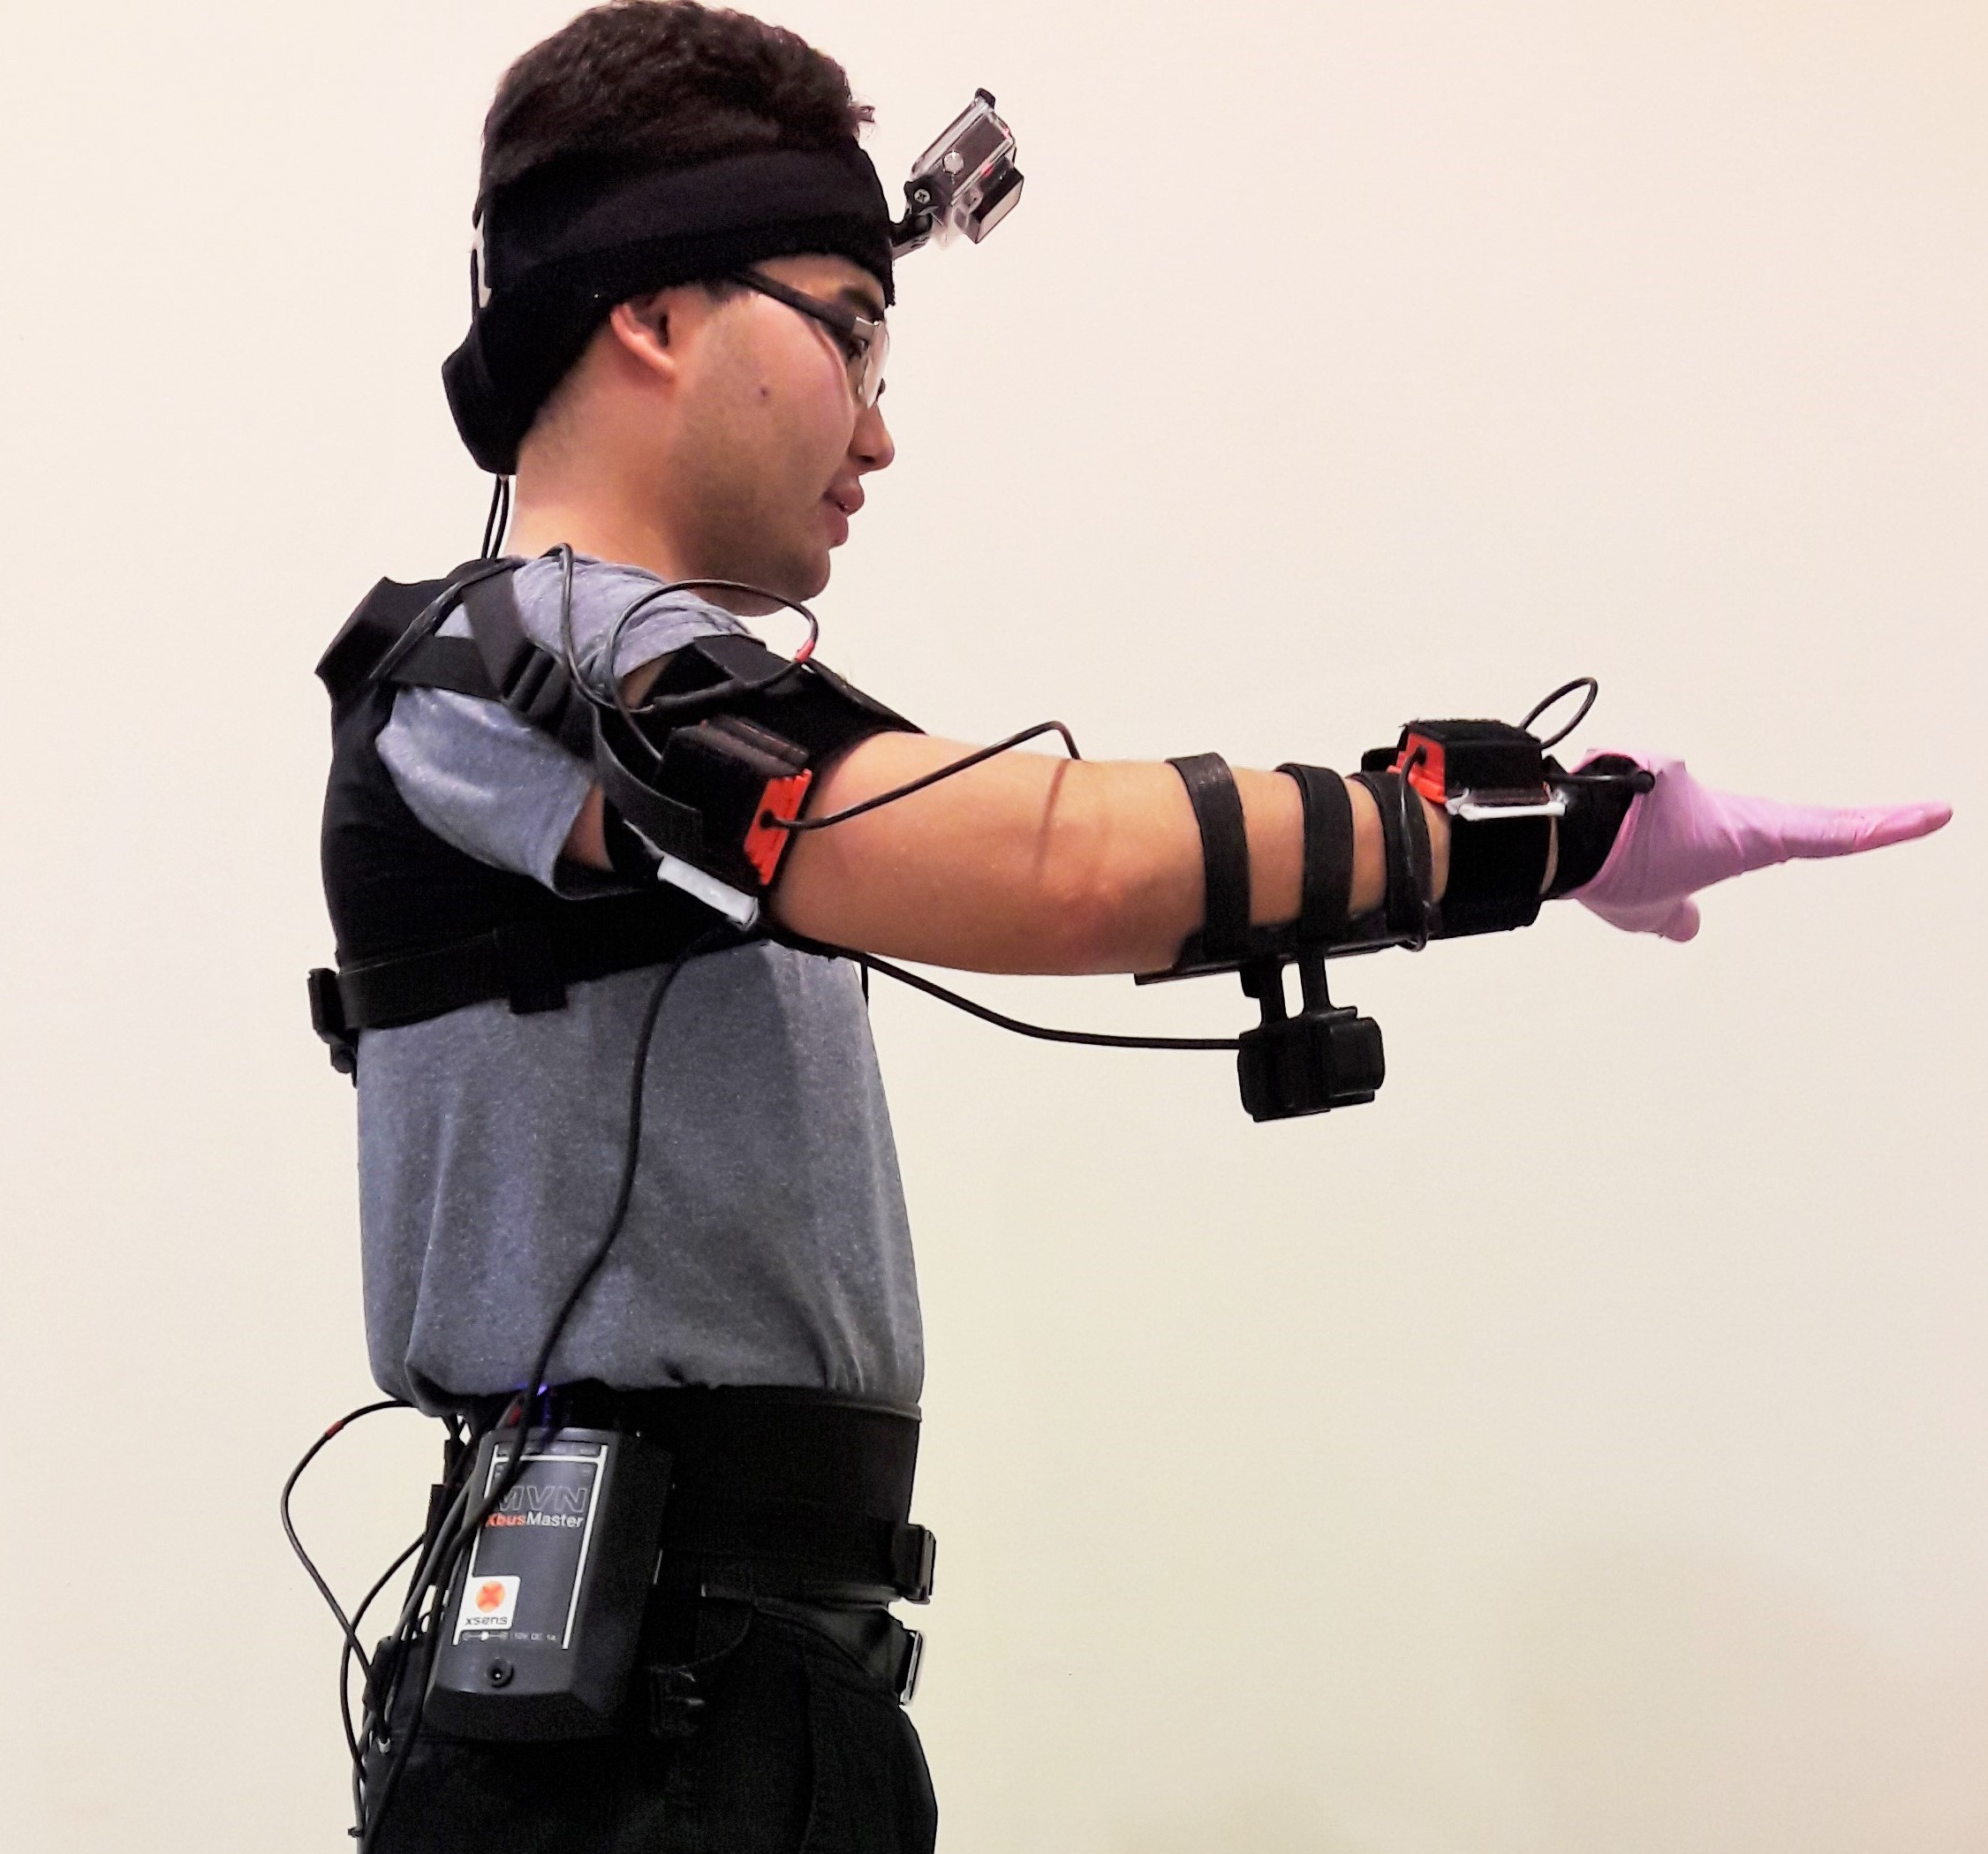
\includegraphics[scale=0.108]{Setup}
\caption{Researcher wearing the setup: head-mounted camera GoPro Hero 4 Silver, upper-body XSENS MVN suit and hand strapped DS325 depth camera.}
\label{fig:setup}
\centering
\end{figure}

\begin{figure}[b]
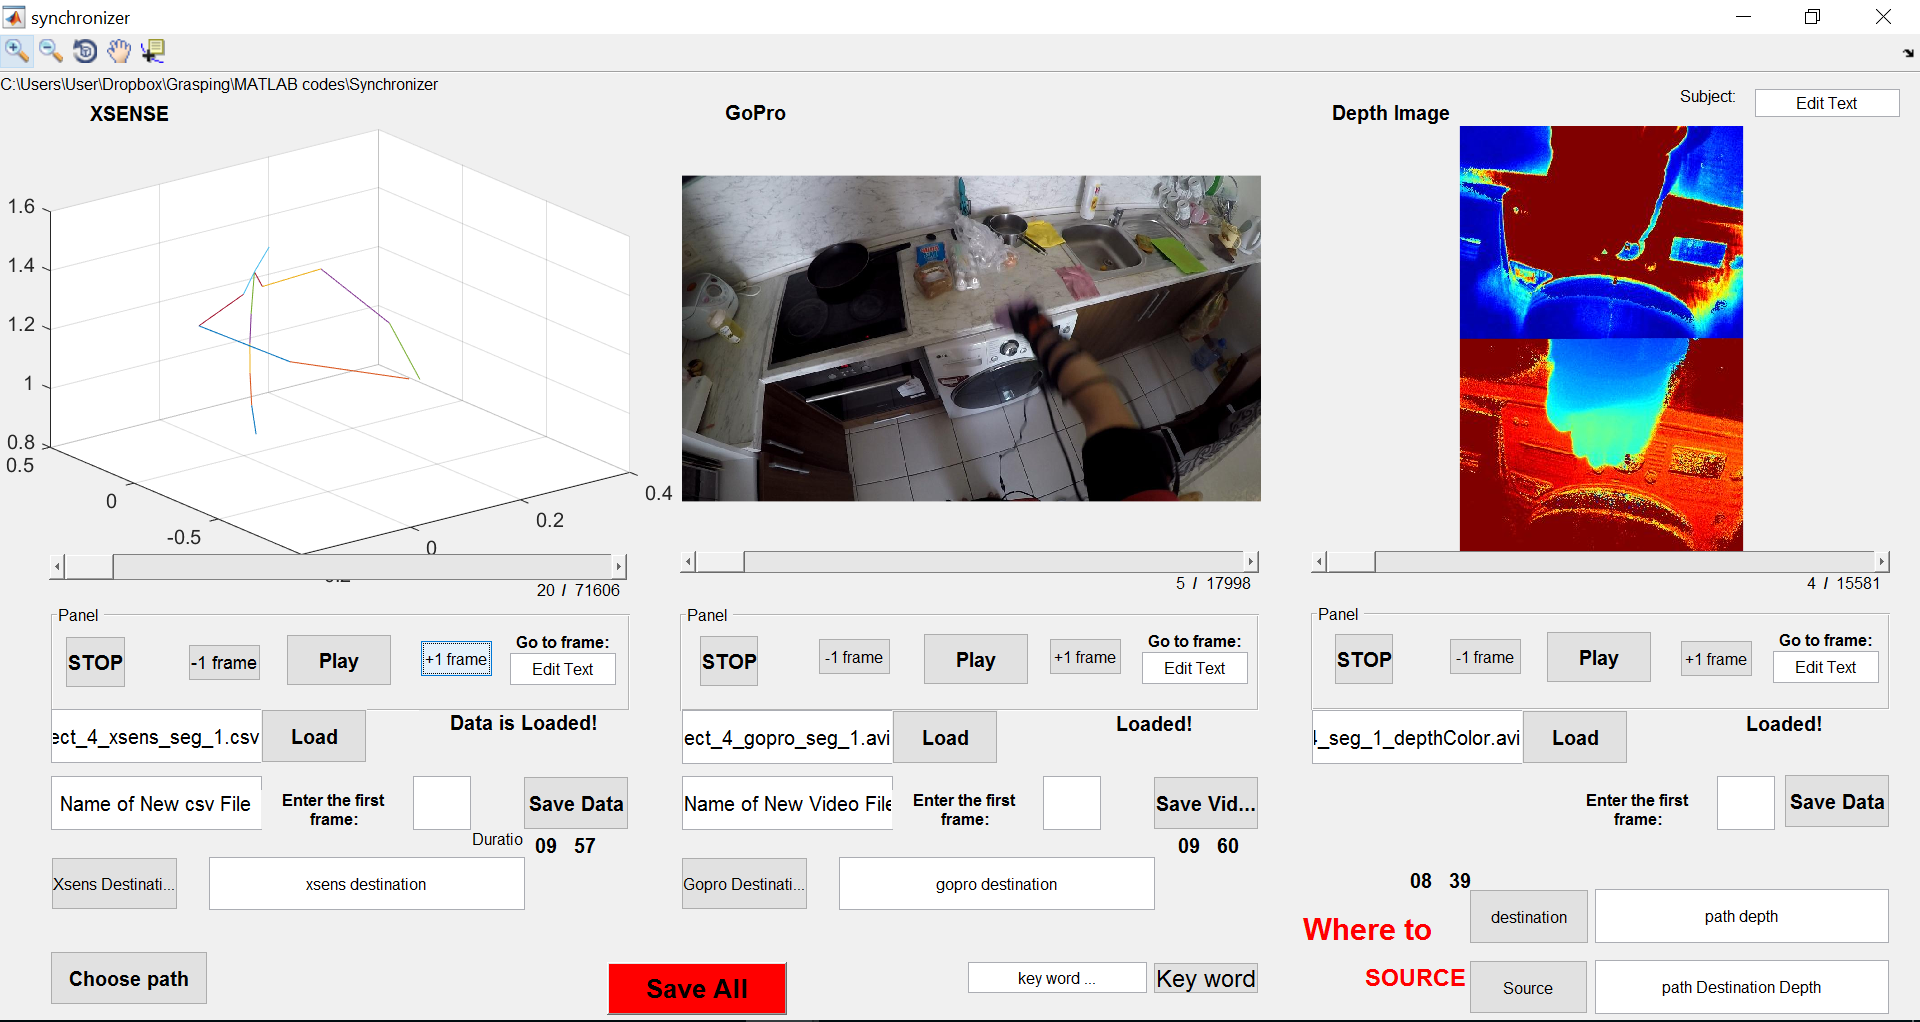
\includegraphics[scale=0.26]{Synchronizer}
\caption{Interface of Synchronization Software containing relevant frames from three channels: XSENS stick man (left), GoPro (middle) and pseudo colored depth/confidence map (right).}
\label{fig:synchronizer}
\centering
\end{figure}

\subsection{Data Acquisition Setup}
	
The multisensory setup consists of three modules enabling acquisition of video, depth and confidence images and upper body inertial motion data. Confidence images are acquired per each depth image from the RGB-Depth camera. They express the magnitude of IR light inflicting on the detector, hence expressing the level of “reliability” of depth measurement in the corresponding pixel of a depth map. 

Video is recorded using a GoPro Hero 4 Silver action camera, weight 83 grams, 59 mm long and 41 mm in height, at 1280 x 720 resolution and 30 frames per second rate. Depth images were acquired using DepthSense RGB-Depth camera, model DS325, of 105 mm x 30 mm x 23 mm dimensions, at 320 x 240 resolution and 30 frames per second rate. The nominal operating range of the RGB-Depth camera is 0.15 m – 1 m. The action camera was mounted to a participant’s head and DepthSense camera was strapped to the dominant hand, hence providing us with high-resolution video capturing wider scene range and high-fidelity depth data more focused on the hand operating range. 

Inertial motion data was recorded using XSENS MVN suit. The suit is comprised of 17 sensors dividing the body into 23 segment labels and 22 joints (see fig. \ref{fig:setup}). In this work we only used the upper body configuration of the XSENS MVN, which includes 11 sensors and omits segments and joints related to legs, feet and toes. Along with gyroscope, accelerometer and magnetometer values, these sensors enable obtaining the position, angular velocity and quaternion data for each body segment. Data from the inertial measurement unit sensors was acquired at 120 frames per second and transmitted wirelessly to the HP EliteBook 8560W laptop (Windows 7 operating system, Intel Core i7 processor). 

Data was recorded in chunks, segments of duration of less than 10 minutes for further annotation convenience. Both laptops were located within 2 - 3 meters range from human participants and did not cause any disturbance or interference with the process. The process was continuously monitored by one of the authors this paper.


\begin{figure}[b]
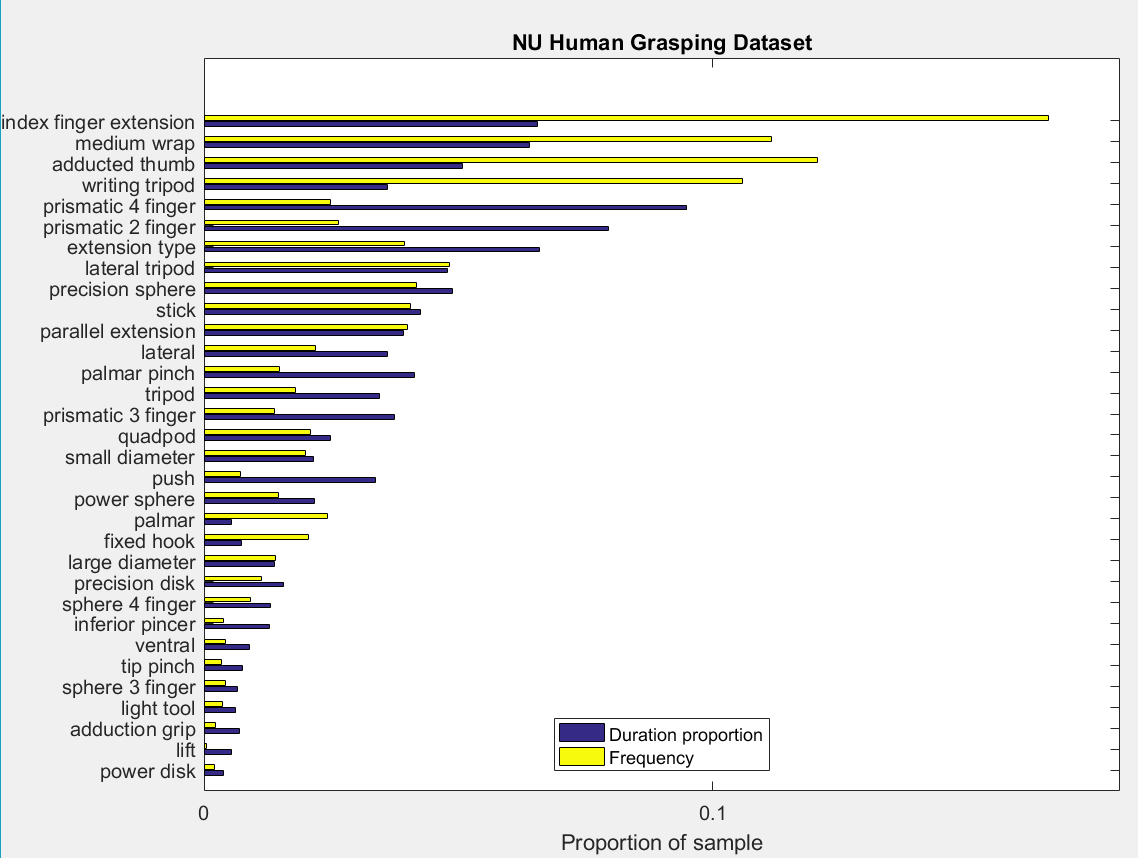
\includegraphics[scale=0.45]{totalStatAll}
\caption{Frequency and Duration proportion of all grasp actions in the NU Grasp Database.}
\label{fig:totalStatAll}
\centering
\end{figure}

\begin{figure}[b]
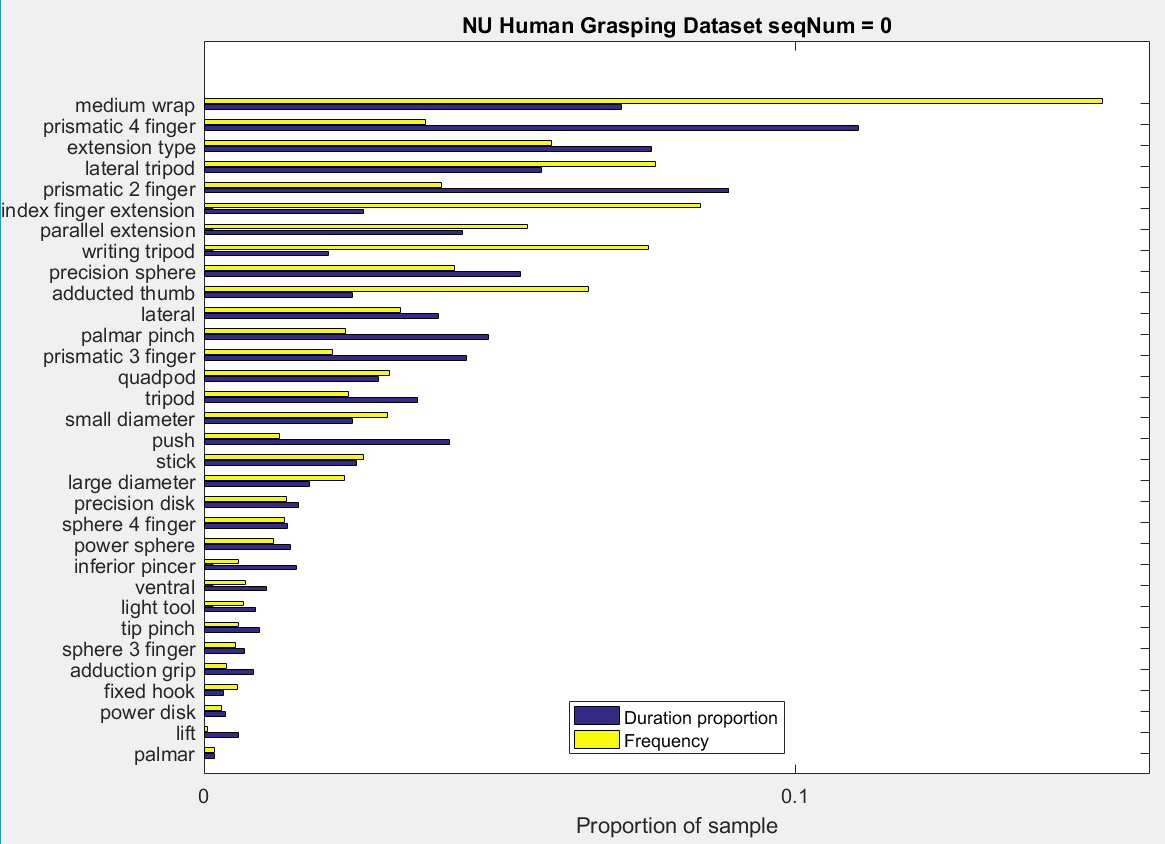
\includegraphics[scale=0.45]{totalStatSeqZero}
\caption{Frequency and Duration proportion of first grasp action in all sequences}
\label{fig:totalStatSeqZero}
\centering
\end{figure}



\subsection{Data Mapping and Annotation}

Three data channels had been recorded asynchronously. Hence, segments of each stream started at different time instant. Additionally, some depth frames were dropped which resulted in non-systematic frame shift. Hence, manual mapping of events by a human expert was required. We created a Matlab graphical user interface program (see fig. \ref{fig:synchronizer}) which allowed visualization of all three streams and the means to access specific frames in each of the channels. The depth stream was visualized using the Matlab’s Jet color map implementation. Annotation was performed by three researchers with engineering background.

We identified discrete grasp actions, similar to the concept of elementary grasp actions used in \cite{IEEEhowto:vergera}.  
Based on our observation of human grasping, we collected multiple grasp actions performed consequently on the same object to the sequence of grasps. Grasp sequence is chronologically numbered stack of grasps.  Starting point of each grasp action was established from the moment a human expert detects a contact to acquire an object. The end point of the action was established when subject released an object or switched to another static grasp. Grasp events identified in the action camera videos were mapped to corresponding frames in the depth and inertial motion data. Each action’s start and end frames were then recorded, respectively. Only the right hand (dominant in each participant) was considered. Time-line outside of the grasps was left untagged. 



There is the total of 3826 grasps identified from the recorded material among which 2922 (4 h 50 m), 564 (1 h 5 m) and 340 ( 28 m) are performed during cooking, housekeeping and laundry activities, respectively. These absolute values reflect both the duration and nature of each activity.

In figures \ref{fig:totalStatAll} and \ref{fig:totalStatSeqZero} are depicted statistical plot of occurrence and duration proportion of all grasps and grasps with 0 sequence number (first grasp in a sequence). The distribution of grasps in both cases has similar pattern. Note that, first grasp in sequence usually deployed to pick up the object and to switch to task related grasp. Therefore, in latter case frequency and durations of precision grasps increased (e.g. prismatic 4/3/2 finger and palmar pinch).











\subsection{Grasp taxonomy and assumptions}

For our list of grasps, we followed the taxonomy provided by Feix et al in \cite{IEEEhowto:feix}, where authors carried out a comprehensive survey and analysis of human grasps. Authors identified 33 distinct types and showed that this list can be reduced to 17 general grasps, when considering only hand configuration. In addition, we added two common non-prehensile grasps - Push and Lift, which do not appear in \cite{IEEEhowto:feix}.

Along with the taxonomy, we followed two assumptions from \cite{IEEEhowto:feix}, during tagging grasp actions. Specifically, we omitted bi-manual tasks, when an action is possible only with application of two hands (e.g. two-hand bedsheet folding). And in-hand motion actions, i.e. movements causing object motion within the hand. 


\begin{figure*}
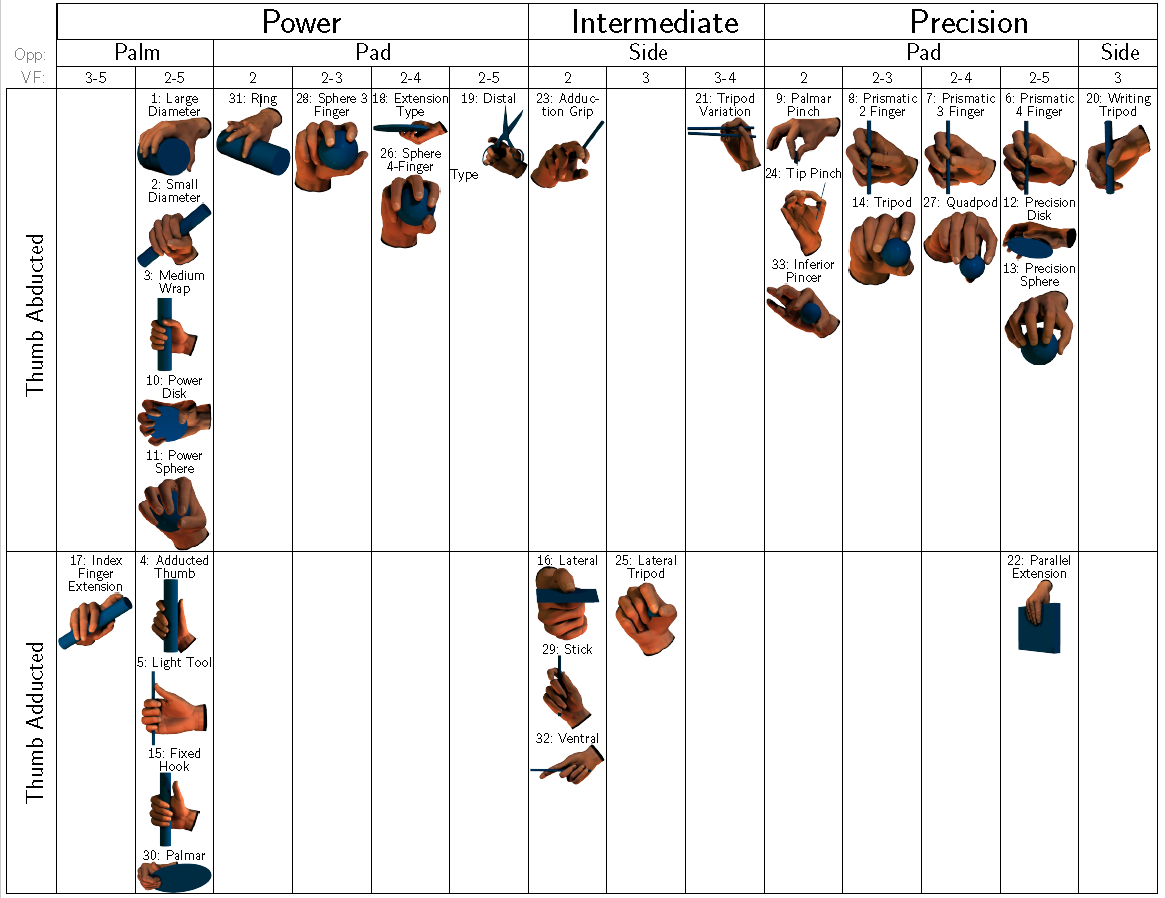
\includegraphics[width=\textwidth,height=13cm]{Taxonomy}
\caption{GRASP taxonomy developed by Thomas Feix, Yale University. The grasps are classified in the columns according to their assignment into power,
intermediate and precision grasp, the opposition type, and the Virtual-Fingers assignment. The assignment of the rows is done be the position of the thumb that can be in an
abducted or adducted position.}
\label{fig:taxonomy}
\centering
\end{figure*}

\subsection{Data description}

As a result of aforementioned procedures, we generated and structured experimental data and corresponding annotation file. The dataset is organized as per human subject such that video, depth, inertial motion data and annotation obtained for each participant are grouped together in a separate folder. Thus, our dataset contains 13 folders with names of participant the data was acquired from. Furthermore, each subject directory contains separate folders for GoPro video files, depth images and inertial motion data. GoPro videos are stored as Audio Video Interleaved (AVI) files, depth and confidence images in the Portable Network Graphics (PNG) format, and inertial motion data as comma separated files. As mentioned in the Methods section, the length of experiments varied across participants and acquisition was performed in 10-minute long segments. This way, for every sensing modality, there might be different number of files available. E.g. if subject 1 experiment lasted for 30 minutes, there will be 3 AVI files in the GoPro videos folder of that subject. At the same time, if subject 2 experiment lasted 40 minutes, there will be 4 AVI video files in the corresponding folder. 

Data acquired from the XSENS motion capture suit, stored in a comma-separated file, contains 227 columns each representing specific inertial measurement taken from an upper body of a subject. The full body XSENS suit contains 17 inertial measurement units (IMU) each comprised of a gyroscope, accelerometer and magnetometer.  There are 22 labeled joints and 23 enumerated body segment labels indicated the origin of the inertial motion data. In our experiments, we used the upper body configuration of the suit, hence omitting number sensors, joints and segment labels, such as upper and lower legs, feet and toes. Upper body configuration provides with 227 sensor and body segment labels, arranged as 227 data columns in the comma-separated file. Specifically, first 150 columns contain the data from 15 segment labels, including Pelvis, Right Hand, Right Forearm, Right Upper Arm, Right Shoulder, Neck, Head, etc. For each segment, the system provides 10 fields - 3 position, 4 quaternion and 3 angular velocity values. Subsequently, there are 77 columns, which contain 3 gyroscope and 4 quaternion values for each of 11 sensors of the upper body suit, such as Pelvis, Head, Right Hand, Right Upper Arm, etc. 

The annotation is provided as a csv file in the root directory of the dataset. There are 13 columns in the annotation file. The file indicates the id of the grasp and the participant it belongs to. In addition, the file identifies the grasp type as identified from the taxonomy, task type as annotated by human experts and start and end frames of the episode to locate them in the GoPro video files. Finally, the annotation describes the grasp properties including opposition type, power level and thumb position. From first to last, the columns represent the values for Grasp ID, Participant ID, Grasp Type, Task Type,  Video File Name, Start Frame, End Frame, Opposition Type, Power level, Virtual Finger, Thumb configuration, Sequence Number, Start Frame (Depth) and End Frame of Depth images. The overall size of the annotated data is 226 GB.


\section{Mining Depth data}

Depth images were applied to a machine learning task. The goal was to learn the state of the hand, whether it is grasping or not. Figure \ref{fig:GraspingNonGrasping} shows pseudo-colored two classes of depth image that trained model supposed to distinguish. First, raw depth images were supplied to Cubic SVM and Bagged Trees classifiers with five fold cross validation which resulted in 83\% and 89\% level of accuracy. Meanwhile, confidence map based filtered depth images improved the accuracy level to 89\% and 92\% respectively. 


\begin{figure*}
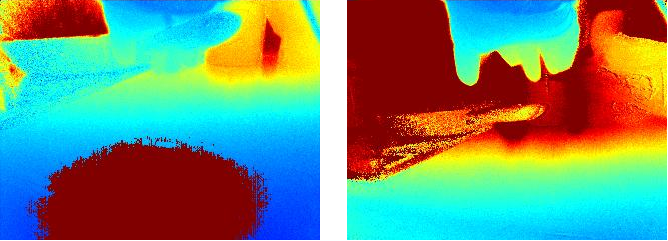
\includegraphics[scale = 1.3]{GraspingNonGrasping}
\caption{Pseudo-colored depth images showing grasping(left) and non-grasping hand(right). }
\label{fig:GraspingNonGrasping}
\centering
\end{figure*}

\begin{figure*}
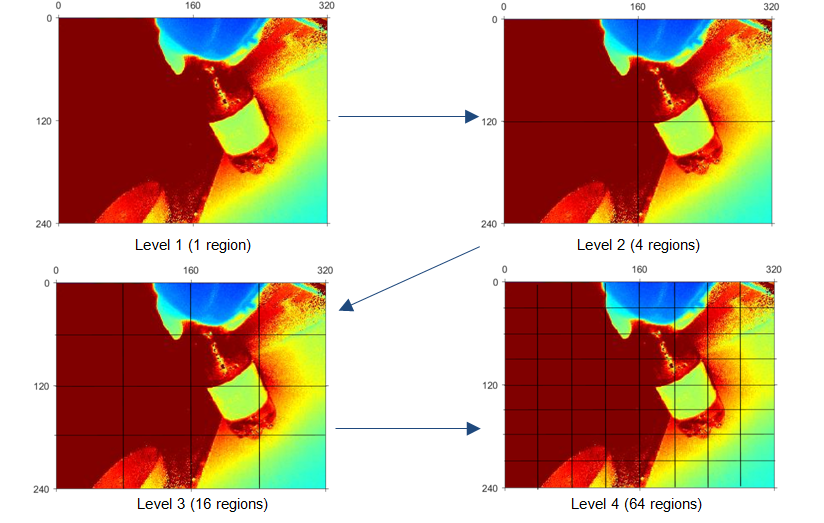
\includegraphics[scale = 1.09]{Mining}
\caption{Recursive quadtree images used for feature extraction }
\label{fig:Mining}
\centering
\end{figure*}



\subsection{Feature Extraction}

Annotated file of RGB video streams provides the moment of contact of the hand with an object. Thus, we assume that frames before the moment of contact are images of non-grasping hand and after are images of grasping hand. Although, number of grasping instances are limited to 3800 (2500 usable, because of grasp sequencing) for this specific task we can supply significantly large amount of data. As a result over 25000 of frames were taken as a training data. 

Features from depth images were acquired by dividing it into uniformly 
sized rectangular regions in quadtree manner. Furthermore, four statistical 
values minimum, maximum, mean and standard deviation from each region were taken 
into account. Depth image is divided into regions in an
iterative manner: first level is the full 320 x 240 pixels image.
This region is then divided into four uniform regions of 160
x 120 pixels. Each of the four obtained regions is divided into
another four uniform rectangles, which provides 16 regions
and 16 + 4 + 1 = 21 total regions at level 3. This process
continues and for levels 4 there are a total of 85, respectively (see Figure 
\ref{fig:Mining}). At every stage
statistical data of each region is extracted and stored in a
vector. With four features obtained from a region, iterations
2, 3, and 4 generate feature vectors of 20, 84, and
340 lengths, respectively.


\subsection{Filtering Depth Images}

Unfortunately, depth cameras have technical limitations in the area they are able to cover. There are cases when data reliability drops as the object goes beyond the the sensibility of the camera. Mainly distortions are introduced due to the reflectivity of the materials being observed. Luckily, DepthSense camera provides us with the confidence map together with the depth images. By assigning values of infrared specter from confidence maps to the depth data, there is a way to test reliability of the recordings. The issue was solved by using normalized confidence map as a filtering mask for corresponding vales in the depth image to obtain higher levels of denoising. This solution was preferred as it is rather fast and requires minimum amount of computations.\cite{IEEEhowto: Saudabayev}  The used formula is as follows:

\begin{equation}
D_{filt}(i,j)=\frac{\sum_{k_i=-l}^{l}\sum_{k_j=-l}^{l}D(i+k_i, j+k_j)\cdot{C(i+k_i, j+k_j)}}{\sum_{k_i=-l}^{l}\sum_{k_j=-l}^{l}C(i+k_i, j+k_j)}
\end{equation}
Where D is the depth image and C is a confidence map matrix.

This approach requires that for each depth frame there is a corresponding confidence map acquired simultaneously. Usage of filtering improved results of mining the depth data.




\section{Conclusion}
Primary contribution of this work is providing sensor rich Human Grasping database consisting arm kinematics and depth image streams. The dataset is available on-line and at the ARMS lab server. 9 hours of RGB video streams were annotated for grasping matter. Moreover, depth streams were synchronized with head mounted camera. Provided the over 3800 grasping instances this database has potential to answer various questions regarding human grasping behavior related to the arm movements and object shapes. 


% further improvements?



\ifCLASSOPTIONcaptionsoff
  \newpage
\fi


\begin{thebibliography}{5}

\bibitem{IEEEhowto:bullock1}
Bullock, Ian M., Thomas Feix, and Aaron M. Dollar. \emph{"The Yale human grasping dataset: Grasp, object, and task data in household and machine shop environments."} The International Journal of Robotics Research 34.3 (2015): 251-255.

\bibitem{IEEEhowto:bullock2}
Bullock, Ian M., et al. \emph{"Grasp frequency and usage in daily household and machine shop tasks."} IEEE transactions on haptics 6.3 (2013): 296-308.

\bibitem{IEEEhowto:cutkosky}
Cutkosky, Mark R. \emph{"On grasp choice, grasp models, and the design of hands for manufacturing tasks."} IEEE Transactions on robotics and automation 5.3 (1989): 269-279.

\bibitem{IEEEhowto:feix}
Feix, Thomas, et al. \emph{"The GRASP taxonomy of human grasp types."} IEEE Transactions on Human-Machine Systems 46.1 (2016): 66-77.


\bibitem{IEEEhowto: Grebenstein} 
Grebenstein, Markus, et al. "The hand of the DLR hand arm system: Designed for interaction." The International Journal of Robotics Research 31.13 (2012): 1531-1555.

\bibitem{IEEEhowto: Saudabayev} 
Saudabayev,Artur, Farabi Kungozhin, Damir Nurseitov, and Huseyin Atakan Varol, “Locomotion Strategy Selection for a Hybrid Mobile Robot Using Time of Flight Depth Sensor,” Journal of Sensors, vol. 2015, Article ID 425732, 14 pages, 2015. doi:10.1155/2015/425732


\bibitem{IEEEhowto:vergera}
Vergara, Margarita, et al. \emph{"An introductory study of common grasps used by adults during performance of activities of daily living."} Journal of Hand Therapy 27.3 (2014): 225-234.

\bibitem{IEEEhowto: Declaration of Helsinki}
World Medical Association. "World Medical Association Declaration of Helsinki: ethical principles for medical research involving human subjects." Journal of postgraduate medicine 48.3 (2002): 206.


\end{thebibliography}


\end{document}


